\chapter{Alternative Synchronization Architectures}
\label{app:async_sync}

\section{Single-Branch Asynchronous Frame Synchronizer}

To resolve the phase ambiguity introduced by the Costas loop without the computational overhead of running multiple parallel $\mathtt{Viterbi}$ decoders, an asynchronous feedback-based frame synchronization algorithm was initially developed and evaluated. 

\begin{figure}[h]
    \centering
    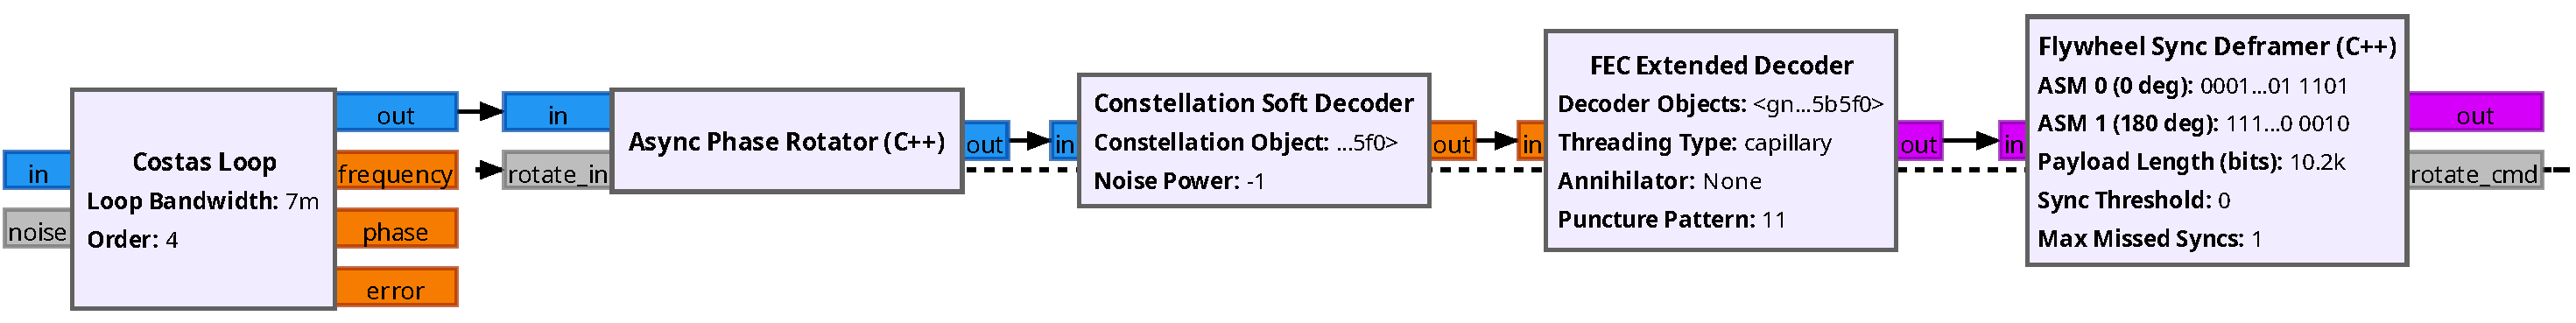
\includegraphics[width=1\textwidth]{figures/Inkscape/flywheel1.pdf} 
    \caption{Receiver architecture with a custom single-branch flywheel algorithm.}
    \label{fig:flywheel_blocks} 
\end{figure}

This alternative architecture prioritizes computational speed and resource efficiency by utilizing only a single $\mathtt{Viterbi}$ decoding pipeline. Because the $\mathtt{Viterbi}$ decoder is transparent to $\pi$-radian phase inversions, the synchronizer can search for both the non-rotated Access Sync Marker (ASM) and its $\pi$-radian inverted counterpart simultaneously. To account for the remaining $\pi/2$ and $3\pi/2$ ambiguities, the algorithm utilizes a feedback loop: if the ASM is not found, it assumes the Costas loop has locked onto an orthogonal phase and sends an asynchronous message to a rotation block to shift the incoming constellation by $90^\circ$.

The logic of this algorithm relies on a four-state machine, illustrated in \Cref{fig:states_async}:

\begin{itemize}
    \item \textcolor{gray}{Search mode}: The $32$-bit preamble (both normal and inverted) is searched for within the incoming bitstream. If a potential preamble is detected, the system transitions to \textit{Check} mode. If no preamble is found within a predefined timeout period, it transitions to \textit{Rotate} mode.
    \item \textcolor{gray}{Check mode}: The algorithm verifies that the subsequent data matches the frame criteria to prevent false positives before fully committing to the lock.
    \item \textcolor{gray}{Lock mode}: The search window jumps by a fixed space equal to the frame length to check for the next preamble. If it is not found, a \texttt{max\_misses} counter is incremented. If this counter overflows, the system assumes a Costas loop phase slip has occurred and transitions to \textit{Rotate} mode.
    \item \textcolor{gray}{Rotate mode}: Triggered by the \texttt{max\_misses} overflow or search timeout, this state sends an asynchronous message to the upstream rotator block to shift the constellation phase by $90^\circ$. Afterward, it immediately returns to \textit{Search} mode.
\end{itemize}

\begin{figure}[h]
    \centering
    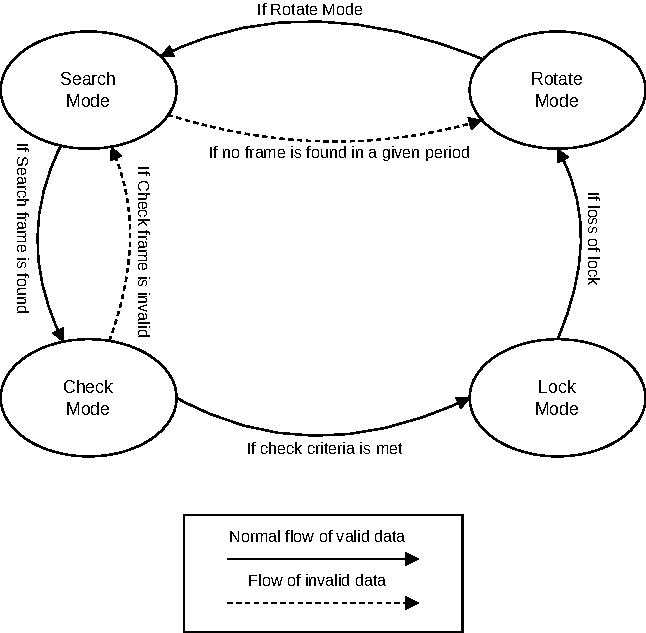
\includegraphics[width=0.65\textwidth]{figures/Inkscape/states.pdf} 
    \caption{State machine diagram for the single-branch asynchronous flywheel algorithm.}
    \label{fig:states_async} 
\end{figure}

\subsection{Performance Limitations and Latency}

While this single-branch approach successfully reduces CPU load, it introduces a critical disadvantage regarding the Bit Error Rate (BER) and Frame Error Rate (FER). Because the message to rotate the constellation is asynchronous, the feedback loop suffers from pipeline latency. 

When a phase slip occurs during \textit{Lock} mode, the system expects a frame but fails to find the preamble. The \texttt{max\_misses} variable increments, and upon overflowing, triggers the \textit{Rotate} state. By the time the asynchronous message reaches the rotation block and the newly rotated symbols propagate through the $\mathtt{Viterbi}$ decoder, several frames of valid data have already been corrupted. Specifically, data is trapped in the $\mathtt{Viterbi}$ input buffer, the decoder's history window, the output buffer, and the synchronizer's own input buffer. In practice, this architectural latency results in a systematic loss of $5$ consecutive frames every time the Costas loop slips.

\begin{figure}[h]
    \centering
    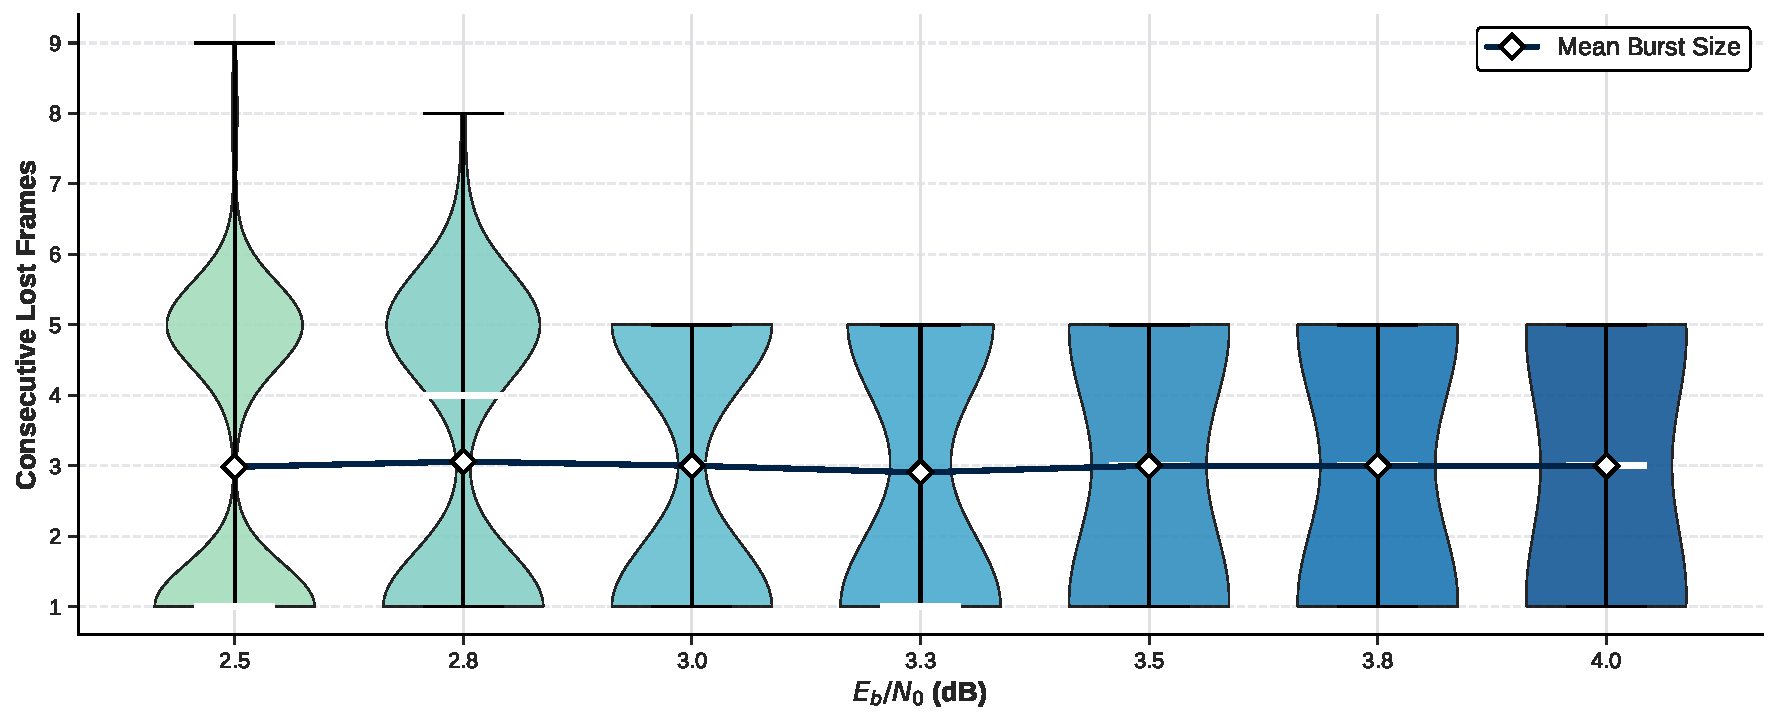
\includegraphics[width=0.8\textwidth]{figures/Inkscape/Doppler_BurstLoss.pdf} 
    \caption{Distribution of Sync Loss Burst Sizes using the asynchronous feedback architecture (Doppler Soft 5m).}
    \label{fig:Comparative_frame_sync_async}
\end{figure}

To mitigate this burst loss, setting \texttt{max\_misses = 0} was considered, which would theoretically reduce the loss from $5$ to $4$ frames by reacting instantly to a single missed ASM. However, empirical testing showed that a single bit error within the $32$-bit ASM due to channel noise is statistically more probable than a genuine Costas loop phase slip. A \texttt{max\_misses} value of $0$ causes the system to erroneously rotate the phase due to minor noise, destroying the lock entirely. Consequently, \texttt{max\_misses} must be maintained at $1$ or higher. 

Ultimately, while the single-branch asynchronous algorithm is computationally lightweight, the inherent pipeline latency and resulting burst frame losses make it unsuitable for links operating at low $E_b/N_0$, justifying the shift to the dual-branch feed-forward architecture described in the main text.